\begin{figure}
    \begin{center}
    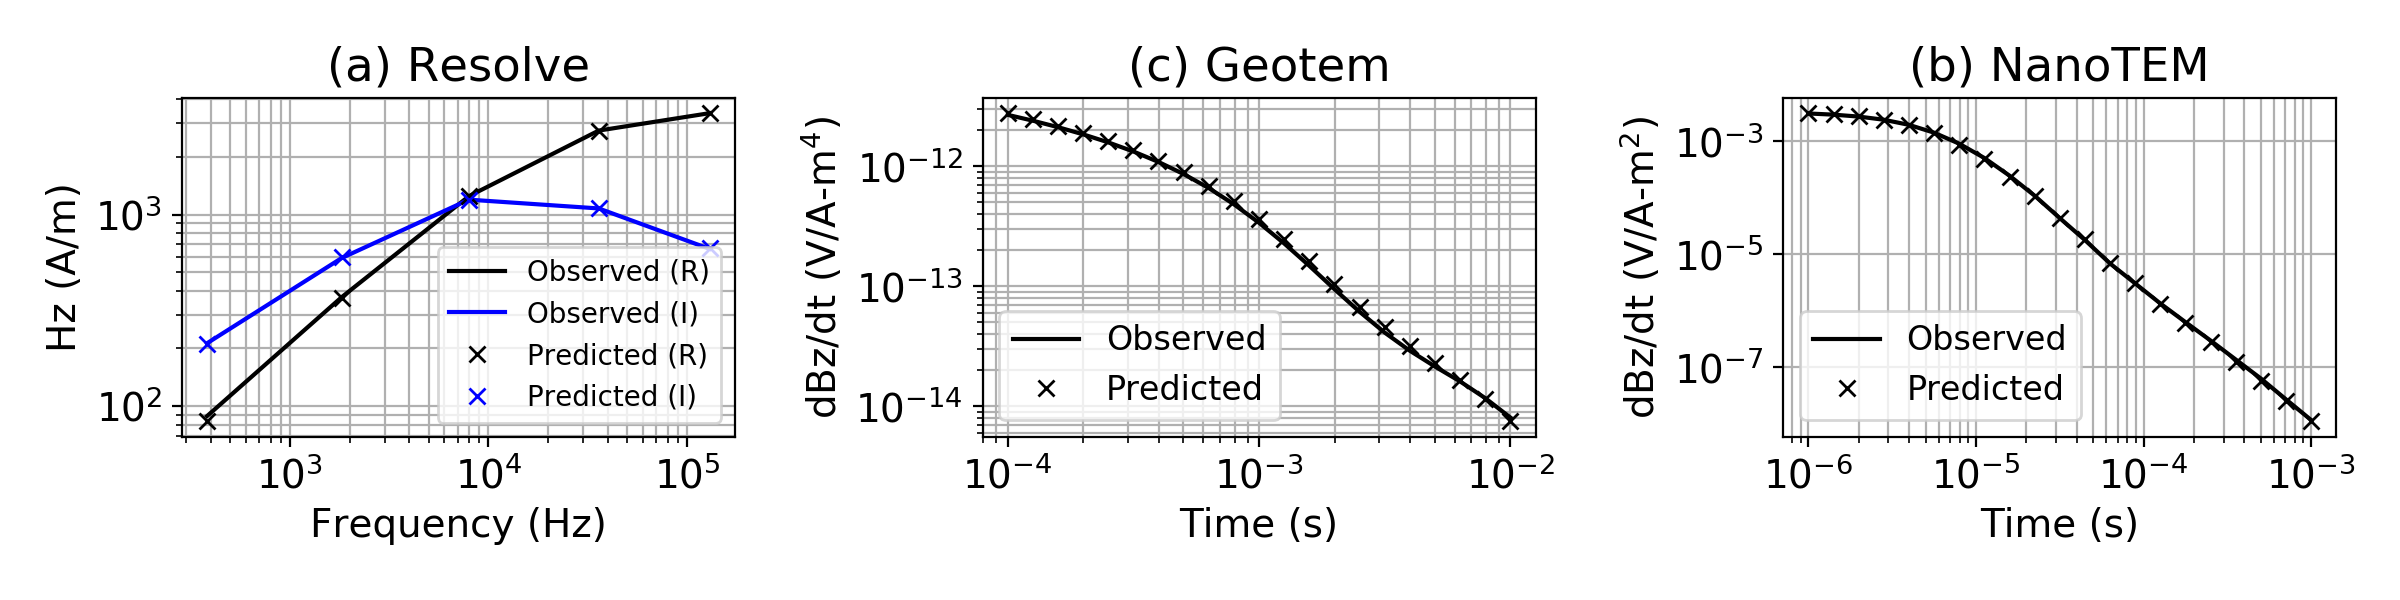
\includegraphics[width=\columnwidth]{figures/obs-vs-pred.png}
    \end{center}
\caption{
    Comparison of observed and predicted data from each of the three inversions: (a) Resolve, (b) Geotem, and (c) NanoTEM. The joint inversion shows a similar level of data fit as those shown here. The black and blue colors distinguish real and imaginary values for the Resolve data. The solid line and cross marks indicate observed and predicted data, respectively.
}
\label{fig:obs-vs-pred}
\end{figure}


